\chapter{Experiments and Results Analysis}
\section{Environment}
The experiment was carried out using an Intel(R) Core(TM) i5-8250U CPU @ 1.60GHz, 1801 Mhz, 4 Core(s), 8 Logical Processor(s), Windows 11 OS, and 8 GB of main memory. The proposed approach was written and executed in Python using the Anaconda Jupyter Notebook.

\section{Dataset Overview}
We conducted experiments with three data sets Iris, Pendigit, and Waveform. We are using the datasets available in sci-kit-learn, which retrieves datasets from the OpenML platform. Description of datasets are:
\begin{enumerate}
    \item \textbf{Iris}: The Iris dataset is a well-known dataset for machine learning and statistics. It includes dimensions for iris blossoms from three different species: Setosa, Versicolor, and Virginica. Each species contains 50 samples, for a total of 150 samples.
    \item \textbf{Pendigits}: The Digits dataset comprises 1,797 instances, each containing 64 properties. These properties correspond to the grayscale values of pixels in an 8x8 picture depicting handwritten numbers. The dataset comprises 10 distinct categories, each representing a numerical number ranging from 0 to 9.
    \item \textbf{ Waveform:} The Waveform dataset comprises artificially generated time-series data employed for binary classification tasks. There are 5,000 instances, each containing 21 numerical properties.
\end{enumerate}

\section{Evaluation Metrics}
The Evaluation metrics that have been used here for quantitative results are Normalized Mutual Information (NMI). \cite{estevez2009normalized}, Silhouette Coefficient (SC). \cite{rousseeuw1987graphical}, Davies-Bouldin Index (DBI) 
 .\cite{davies1979}.
\begin{enumerate}
    \item \textbf{Normalized Mutual Information (NMI):} NMI is a metric for evaluating clustering quality against ground truth and comparing clustering results from various techniques. NMI is the normalized MI score, hence the values are between 0 and 1. The higher an algorithm's NMI value, the better it is for clustering.
    \item \textbf{Silhouette Coefficient (SC):} SC is used to determine how well one cluster is segregated from another. It ranges from -1 to one. Higher SC values imply more well-divided clusters. 
    \item \textbf{Davies-Bouldin Index (DBI):} DBI is also used to measure how well clusters are separated based on the ratio of distances within the cluster and between the clusters. If the distance between the clusters is greater, then the ratio will decrease; therefore, a lower DBI value will signify well-separated clusters.
\end{enumerate}
\section{Hyperparameter Analysis}
LAPUMAP involves hyperparameters: $min\_dist$, $n\_neighbours$, $\hat{k}$ and $\lambda$, which significantly affect the quality of visualization. For particular values of $n\_neighbours$, a decrease in $min\_dist$ gives better cluster separation and increases NMI. With a particular value of $n\_neighbours$ and $min\_dist$, we have to increase $\lambda$ to increase NMI. $\hat{k}$ determines the number of clusters that will form in low dimensional space if we give $\hat{k}$ less than $k$ then there is a possibility of overlapping among the clusters if $\hat{k}$ is more than k then more number of meaningless clusters will form.  
\section{Results}
We have embedded Iris, Pendigits, and Waveform datasets in low dimensional space, i.e., in 2D space using tSNE, UMAP, LAPtSNE, and UMAP to compare our approach both in quantitative measure and qualitative measures. Below are the visualization and metrics measures observed.
\begin{figure}[H]
    \centering
    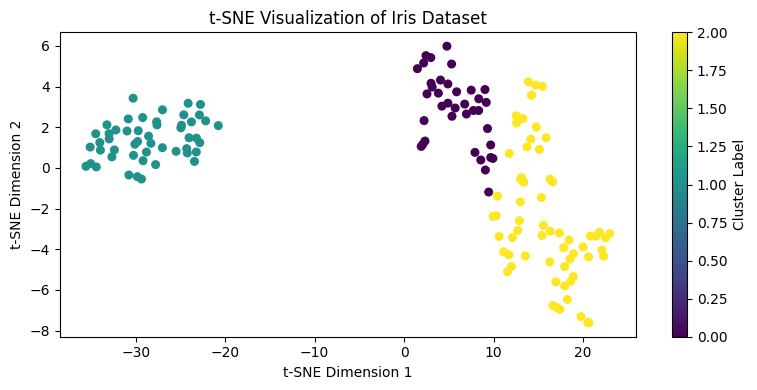
\includegraphics[width=0.7\textwidth]{images/tSNEonIris2.png} % Adjust the width as needed
    \caption{tSNE on Iris}
    \label{fig:1}
\end{figure}
\begin{figure}[H]
    \centering
    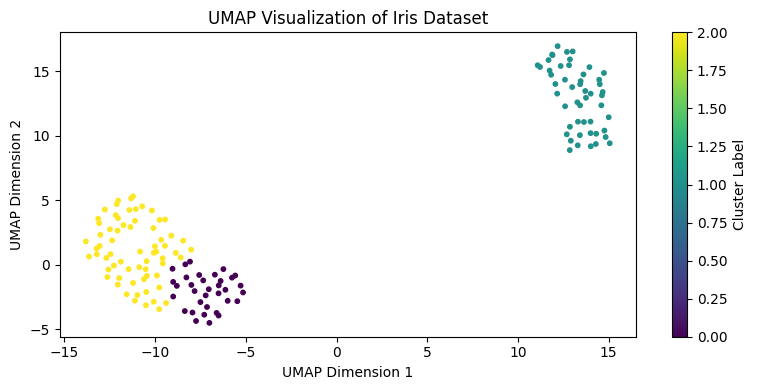
\includegraphics[width=0.7\textwidth]{images/UMAP on Iris1.png} % Adjust the width as needed
    \caption{UMAP on Iris}
    \label{fig:2}
\end{figure}
\begin{figure}[H]
    \centering
    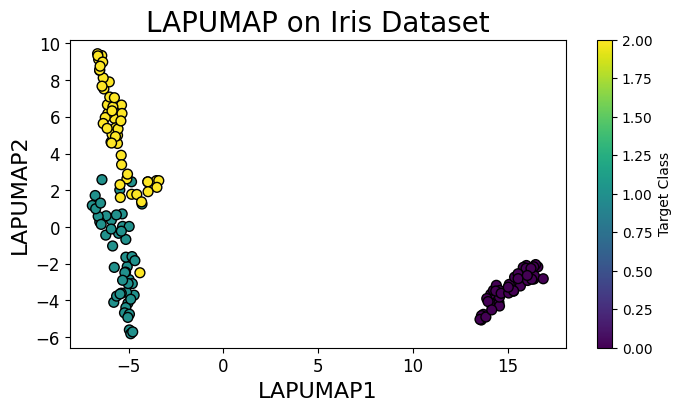
\includegraphics[width=0.7\textwidth]{images/LAPUMAPonIris.png} % Adjust the width as needed
    \caption{LAPUMAP on Iris}
    \label{fig:3}
\end{figure}
\begin{figure}[H]
    \centering
    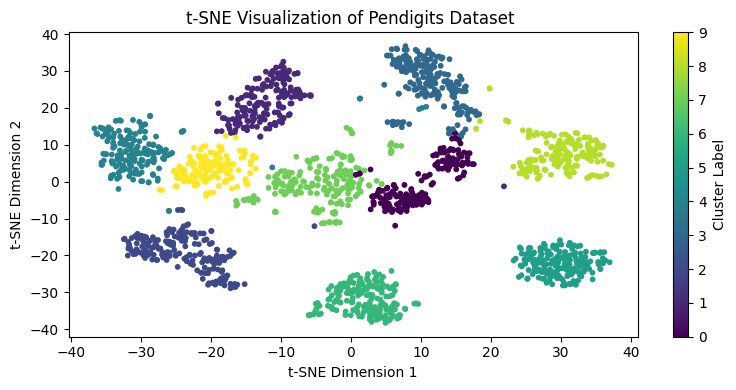
\includegraphics[width=0.7\textwidth]{images/tSNEonPendigits2.png} % Adjust the width as needed
    \caption{tSNE on Pendigits}
    \label{fig:4}
\end{figure}
\begin{figure}[H]
    \centering
    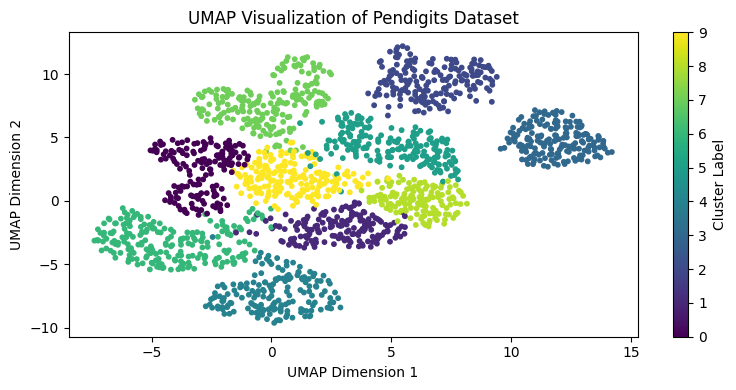
\includegraphics[width=0.7\textwidth]{images/UMAPonPendgits2.png} % Adjust the width as needed
    \caption{UMAP on Pendigits}
    \label{fig:5}
\end{figure}
\begin{figure}[H]
    \centering
    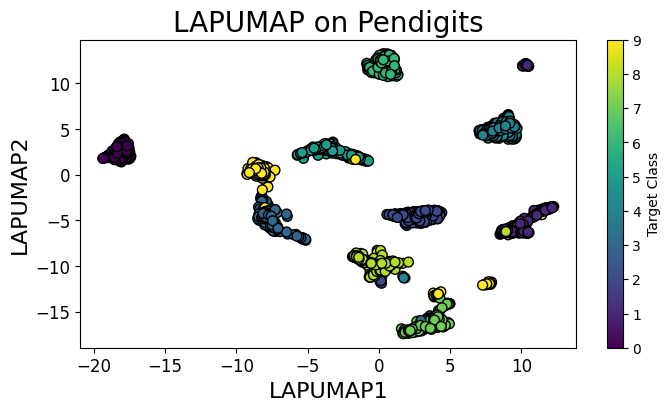
\includegraphics[width=0.7\textwidth]{images/LAPUMAP on Pendigits.png} % Adjust the width as needed
    \caption{LAPUMAP on Pendigits}
    \label{fig:6}
\end{figure}
\begin{figure}[H]
    \centering
    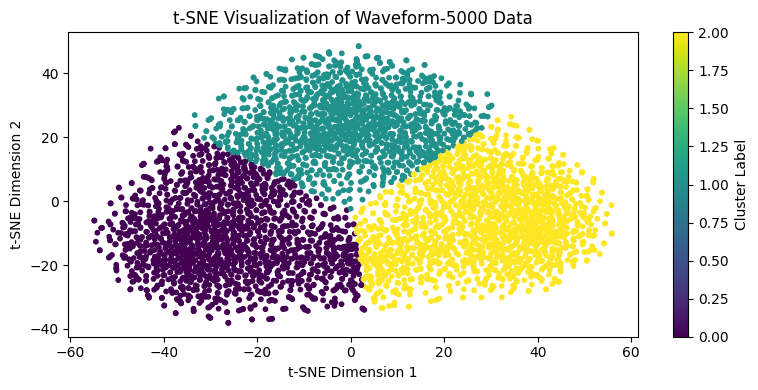
\includegraphics[width=0.7\textwidth]{images/tSNEonWaveform1.png} % Adjust the width as needed
    \caption{tSNE on Waveform}
    \label{fig:7}
\end{figure}
\begin{figure}[H]
    \centering
    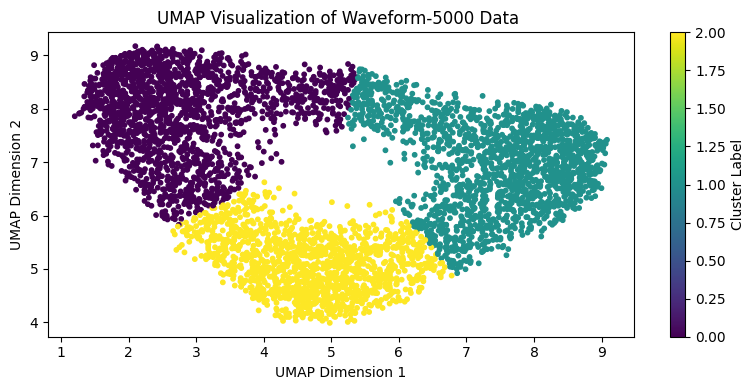
\includegraphics[width=0.7\textwidth]{images/UMAP on Waveform1.png} % Adjust the width as needed
    \caption{UMAP on Waveform}
    \label{fig:8}
\end{figure}
\begin{figure}[H]
    \centering
    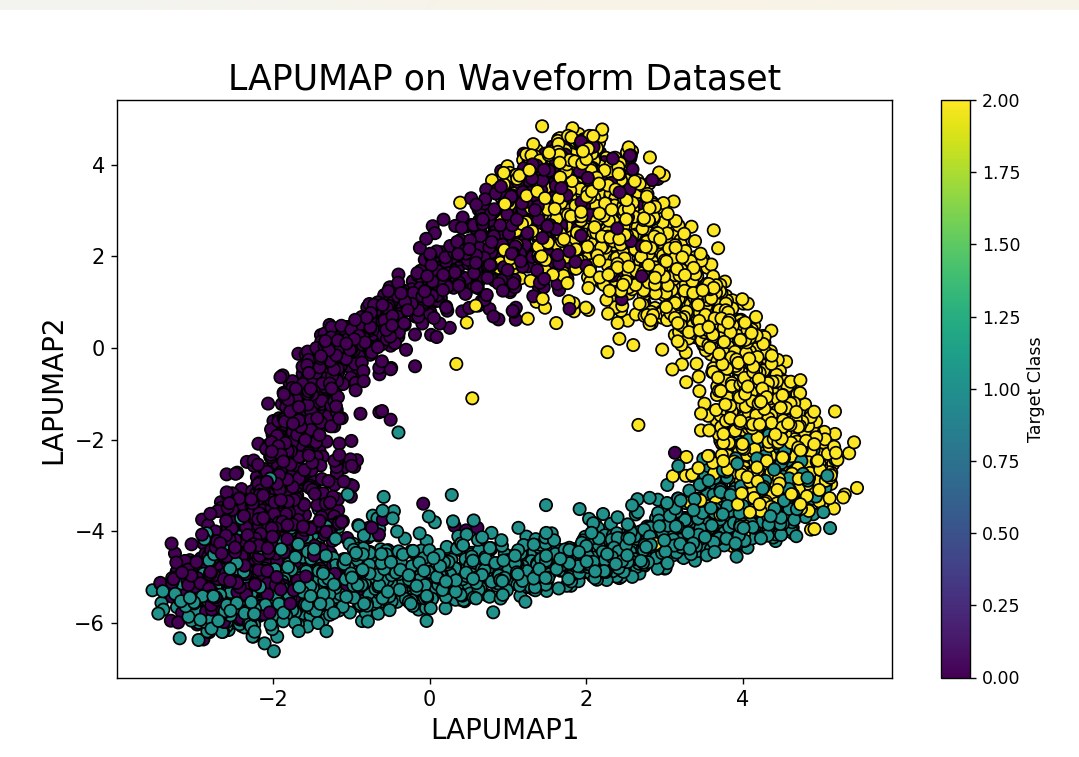
\includegraphics[width=0.7\textwidth]{images/LAPUMAP on WAVEFORM1.png} % Adjust the width as needed
    \caption{LAPUMAP on Waveform}
    \label{fig:9}
\end{figure}


\begin{table}[H]
    \centering
    \begin{tabular}{lccccc}
        \toprule
       \textbf{Datasets} & \textbf{Metrics} & \textbf{LAPUMAP} & \textbf{LAPtSNE} & \textbf{UMAP} & \textbf{tSNE} \\
        \midrule
        Iris &NMI & 0.8056 & - & 0.7560 & 0.7507 \\
        Iris &SC  & 0.6699 & - & 0.5967& 0.6284 \\
        Iris &DBI & 0.4438& - & 0.5986 & 0.4894\\
        \midrule
        Pendigits &NMI & 0.92254& - & 0.8947& 0.8859 \\
        Pendigits &SC  & 0.7786& -& 0.4737& 0.5636 \\
        Pendigits &DBI & 0.2960 & - & 0.6941 & 0.6143\\
        \midrule
        Waveform &NMI & 0.37058 & - & 0.3682& 0.3610\\
        Waveform &SC  & 0.55148& - & 0.5308& 0.4651\\
        Waveform &DBI & 0.59332& -& 0.6274 & 0.7357\\
        
        \bottomrule
    \end{tabular}
    \caption{Quantitative comparison of different dimensionality reduction techniques.}
    \label{tab:dimensionality-reduction-detailed}
\end{table}
\section{Result Analysis}
From Table 5.1 we can see the NMI, and SC values for LAPUMAP are greater than those of UMAP and tSNE, and the values of DBI are less than those of UMAP and tSNE. We know that NMI and SC values should be greater for an algorithm and DBI should be less than other algorithms as mentioned by Estévez et al. .\cite{estevez2009normalized}, Rousseeuw et al. \cite{rousseeuw1987graphical}, and Davies et al.\cite{davies1979} to say that algorithm is superior in terms of clustering. Therefore from these quantitative measures, it is clear that LAPUMAP is superior. If we see the visualizations obtained by tSNE, UMAP, and  LAPUMAP we can say visualization quality is also better using the LAPUMAP, as clusters formed using  LAPUMAP are compact compared to other techniques. LAPUMAP also preserves local and global structures.